\documentclass[11pt]{article}
\usepackage[margin=0.82in]{geometry}
\usepackage{amsmath,amssymb,bm,booktabs,array}
\usepackage{xcolor,graphicx,tikz}
\usetikzlibrary{arrows.meta,positioning,shapes.geometric}
\usepackage[most]{tcolorbox}
\usepackage{enumitem,fancyhdr,hyperref,microtype}
\graphicspath{{../../results/gas_dynamics_week8/}}
\definecolor{navy}{HTML}{17365D}
\definecolor{blue}{HTML}{2F75B5}
\definecolor{teal}{HTML}{2A9D8F}
\definecolor{gold}{HTML}{E9A23B}
\definecolor{red}{HTML}{C44536}
\definecolor{lightblue}{HTML}{EAF3F8}
\definecolor{lightgold}{HTML}{FFF6E6}
\hypersetup{colorlinks=true,linkcolor=navy,urlcolor=blue,citecolor=navy}
\pagestyle{fancy}\fancyhf{}
\lhead{M\&I-ENG 690A -- AI in Fluid Mechanics}\rhead{Week 8 Extension}\cfoot{\thepage}
\setlength{\headheight}{14pt}
\setlist{itemsep=3pt,topsep=4pt}
\newtcolorbox{learningbox}{colback=lightblue,colframe=blue,title=Learning checkpoint,fonttitle=\bfseries}
\newtcolorbox{warningbox}{colback=lightgold,colframe=gold,title=Important distinction,fonttitle=\bfseries}
\newtcolorbox{evidencebox}{colback=white,colframe=navy,title=Evidence gate,fonttitle=\bfseries}
\newtcolorbox{decisionbox}{colback=teal!6,colframe=teal,title=Decision rule,fonttitle=\bfseries}
\newcommand{\Ma}{\mathrm{Ma}}
\newcommand{\Rey}{\mathrm{Re}}
\newcommand{\RelLtwo}{\varepsilon_{L_2}}

\begin{document}
\hypersetup{pageanchor=false}
\begin{titlepage}
\centering\vspace*{0.9cm}
{\color{navy}\rule{\textwidth}{2pt}}\\[0.5cm]
{\Huge\bfseries Gas Dynamics Before\\[0.18cm]Scientific Machine Learning\par}
\vspace{0.35cm}{\Large Exact Relations, Branch-Aware Inversion, and Evidence-Based Surrogates\par}
\vspace{0.35cm}{\large Week 8 Extension Lecture Notes\par}
\vspace{0.5cm}{\color{navy}\rule{\textwidth}{2pt}}\\[0.9cm]
{\Large M\&I-ENG 690A -- AI in Fluid Mechanics\par}
\vspace{0.25cm}{\large Summer 2026\par}
\vfill
\begin{tcolorbox}[colback=lightblue,colframe=blue,width=0.92\textwidth]
\textbf{Central question.} When an exact compressible-flow relation or a bracketed root is already available, what evidence is required before a neural surrogate is scientifically useful?
\end{tcolorbox}
\vfill{\large Instructor: Ehsan Roohi\par}
\end{titlepage}

\hypersetup{pageanchor=true}
\pagenumbering{roman}
\tableofcontents\newpage
\pagenumbering{arabic}

\section{Position in the Course}
Weeks 1--7 establish numerical validation, kinetic sampling, supervised learning,
operator learning, controlled research protocols, and unsteady cylinder wakes.
Week 8 adds compressible-flow physics only after students have learned to separate
a numerical label, a validation target, and a learned approximation.

This module connects three public repositories while preserving their distinct
scientific roles:
\begin{center}
\begin{tabular}{p{0.27\textwidth}p{0.30\textwidth}p{0.32\textwidth}}
\toprule
Source & Role in Week 8 & Claim boundary \\
\midrule
\href{https://github.com/Ehsan-Roohi/Introduction-to-Compressible-Flows}{Compressible-flow book code} & nine chapter-aligned classical notebooks & teaching solvers; analytical and conservation-law checks remain primary \\
\href{https://github.com/Ehsan-Roohi/GasDynamicsSciML}{GasDynBench} & five exact/inverse benchmarks, matched baselines, and frozen evidence & interpretable inverse benchmark; not a replacement for CFD \\
\href{https://github.com/Ehsan-Roohi/SU2-Diamond-Airfoil-Verification}{SU2 diamond-airfoil code} & bridge to multidimensional shock-capturing CFD & one qualified $\alpha=0$ Euler teaching case; eight other cases remain unverified \\
\bottomrule
\end{tabular}
\end{center}

The teaching narrative is aligned with the author-supplied revised manuscript
\emph{Physics-Guided Neural Surrogates for Canonical Compressible Thermal-Fluid
Relations} (manuscript \texttt{AITF-D-26-00044R1}). A revision identifier is
not evidence of acceptance; executable claims remain tied to the frozen public
repository, machine-readable tables, and tests.

\begin{learningbox}
By the end of Week 8, a student should be able to:
\begin{enumerate}
\item identify the governing relation, physical domain, and branches before defining an ML input/output map;
\item compute Rayleigh, Fanno, oblique-shock, nozzle-shock, and shock-tube references;
\item distinguish algebraic evaluation, bracketed inversion, ODE integration, and multidimensional CFD;
\item demonstrate why hiding branch identity produces an ill-posed regression;
\item compare a physics-guided MLP with exact evaluation and interpolation under matched information;
\item test physical bounds, closure residuals, edge generalization, storage, and timing; and
\item state precisely when the neural model helps and when a classical method remains preferable.
\end{enumerate}
\end{learningbox}

\section{Compressible-Flow Foundations}
For a calorically perfect gas,
\begin{equation}
p=\rho RT,\qquad a=\sqrt{\gamma RT},\qquad \Ma=\frac{|\bm u|}{a}.
\end{equation}
The inviscid conservation laws in differential form are
\begin{align}
\frac{\partial \rho}{\partial t}+\nabla\cdot(\rho\bm u)&=0,\\
\frac{\partial (\rho\bm u)}{\partial t}
+\nabla\cdot(\rho\bm u\otimes\bm u+p\bm I)&=0,\\
\frac{\partial (\rho E)}{\partial t}
+\nabla\cdot[(\rho E+p)\bm u]&=0.
\end{align}
For one-dimensional isentropic changes, stagnation properties obey
\begin{align}
\frac{T_0}{T}&=1+\frac{\gamma-1}{2}\Ma^2,\\
\frac{p_0}{p}&=\left(1+\frac{\gamma-1}{2}\Ma^2\right)^{\gamma/(\gamma-1)}.
\end{align}

\begin{warningbox}
A relation can be numerically smooth and still be non-invertible without a
branch label. Sonic points, shock detachment, internal-shock bounds, and contact
compatibility define the topology of the learning problem.
\end{warningbox}

\subsection{Four computational levels}
\begin{center}
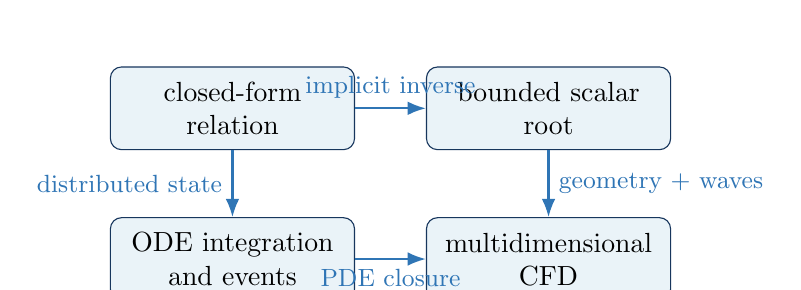
\begin{tikzpicture}[node distance=0.85cm and 0.9cm,>=Latex]
\tikzset{box/.style={draw=navy,rounded corners,minimum width=3.1cm,minimum height=1.05cm,align=center,fill=lightblue}}
\node[box] (a) {closed-form\\relation};
\node[box,right=of a] (b) {bounded scalar\\root};
\node[box,below=of a] (c) {ODE integration\\and events};
\node[box,right=of c] (d) {multidimensional\\CFD};
\draw[->,thick,blue] (a)--node[above,font=\small]{implicit inverse}(b);
\draw[->,thick,blue] (a)--node[left,font=\small]{distributed state}(c);
\draw[->,thick,blue] (b)--node[right,font=\small]{geometry + waves}(d);
\draw[->,thick,blue] (c)--node[below,font=\small]{PDE closure}(d);
\end{tikzpicture}
\end{center}
The baseline must match the level. A neural network should not be compared only
with a slow generic optimizer when a closed-form relation or accurate lookup table exists.

\section{Five Canonical Reference Families}
Figure~\ref{fig:physics-map} shows the exact maps used before learning.
\begin{figure}[ht]
\centering
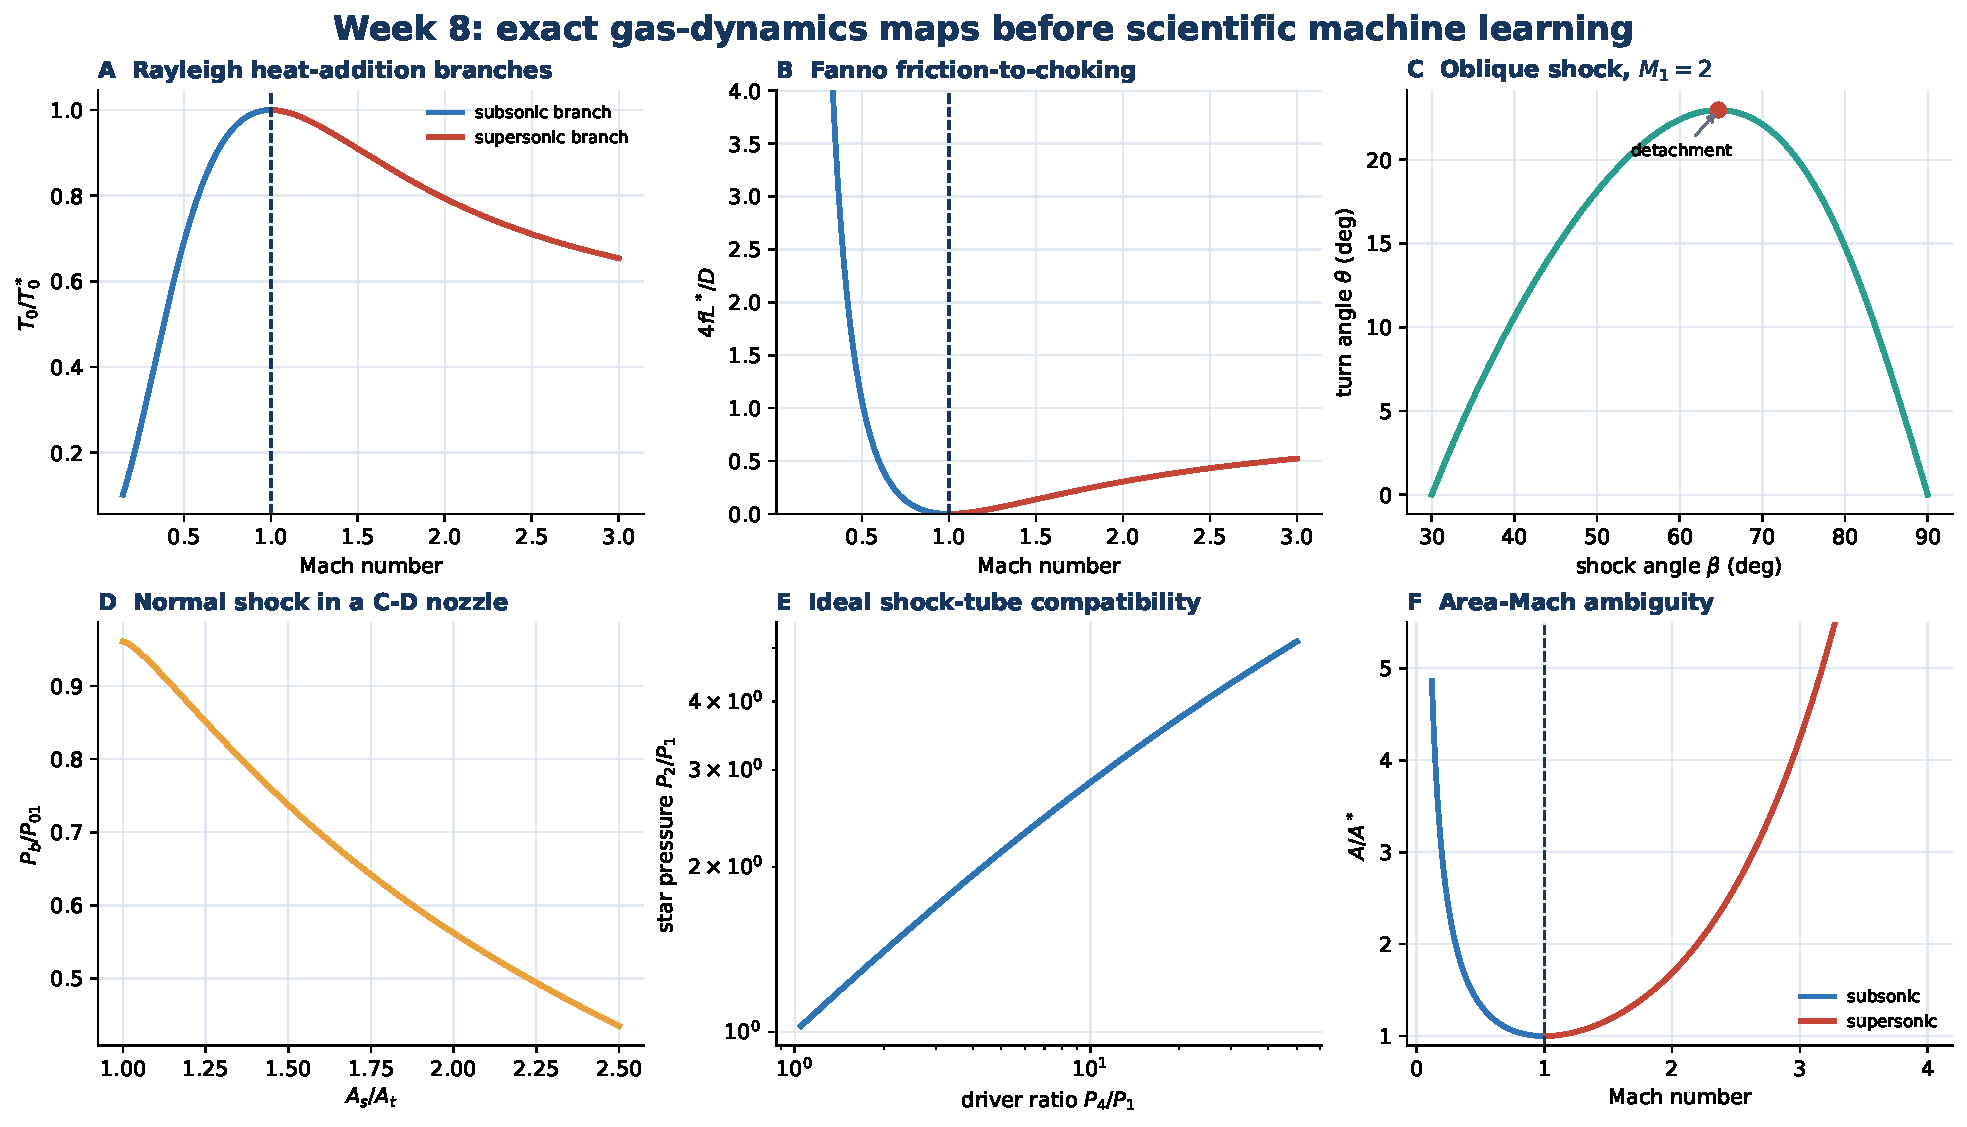
\includegraphics[width=\textwidth]{week8_exact_physics.pdf}
\caption{Exact gas-dynamics maps generated by the FlowMLLab Week-8 module. Dashed sonic lines and turning-point geometry expose the branches that an inverse model must retain.}
\label{fig:physics-map}
\end{figure}

\subsection{Rayleigh flow: heat transfer and sonic choking}
For steady, frictionless, constant-area flow with heat transfer, the sonic
reference ratios include
\begin{align}
\frac{T}{T^*}&=\frac{(1+\gamma)^2\Ma^2}{(1+\gamma\Ma^2)^2},&
\frac{p}{p^*}&=\frac{1+\gamma}{1+\gamma\Ma^2},\\
\frac{T_0}{T_0^*}&=\frac{T}{T^*}
\frac{1+\tfrac12(\gamma-1)\Ma^2}{\tfrac12(\gamma+1)}.
\end{align}
The inverse $T_0/T_0^*\mapsto\Ma$ has subsonic and supersonic roots. The
static ratio $T/T^*$ reaches its maximum at $\Ma=1/\sqrt{\gamma}$, so splitting
that inverse at $\Ma=1$ is inconsistent. Week 8 therefore uses the stagnation
temperature ratio for a clean sonic branch split.

\subsection{Fanno flow: friction length to choking}
For adiabatic constant-area flow with friction,
\begin{equation}
\frac{4fL^*}{D}=\frac{1-\Ma^2}{\gamma\Ma^2}
+\frac{\gamma+1}{2\gamma}
\ln\left[\frac{(\gamma+1)\Ma^2}{2+(\gamma-1)\Ma^2}\right].
\end{equation}
The quantity is nonnegative and vanishes at the sonic state. The subsonic
branch has an unbounded upstream friction length as $\Ma\rightarrow0$, while the
supersonic branch approaches a finite limit. A bounded output transform can
enforce nonnegativity, but it cannot replace a domain check.

\subsection{Oblique shocks: weak and strong attached roots}
The theta-beta-M relation is
\begin{equation}
\tan\theta=2\cot\beta\,
\frac{\Ma_1^2\sin^2\beta-1}
{\Ma_1^2(\gamma+\cos2\beta)+2}.
\end{equation}
For $0<\theta<\theta_{\max}$, weak and strong roots exist on opposite sides of
the detachment maximum. At $\theta_{\max}$ they coalesce. Above it, no attached
root exists. A single naive regressor trained on both roots learns their average,
which is generally neither physical branch.

\subsection{Normal shock inside a converging-diverging nozzle}
The isentropic area relation is
\begin{equation}
\frac{A}{A^*}=\frac{1}{\Ma}
\left[\frac{2}{\gamma+1}
\left(1+\frac{\gamma-1}{2}\Ma^2\right)\right]^{\frac{\gamma+1}{2(\gamma-1)}}.
\end{equation}
It also has subsonic and supersonic branches. An internal normal shock maps
$A_s/A_t$ to $p_b/p_{01}$ through upstream isentropic acceleration, the normal
shock jump, and downstream subsonic diffusion. The inverse is bracketed inside
\begin{equation}
1 < \frac{A_s}{A_t} < \frac{A_e}{A_t}.
\end{equation}
The geometry supplies a hard output bound for both root solvers and learned models.

\subsection{Shock-tube pressure compatibility}
The incident shock and driver expansion must produce the same pressure and
velocity at the contact surface. The equal-gas relation is implicit in
$p_2/p_1$ and is solved with a bracketed root. The generalized benchmark varies
\begin{equation}
\left(\frac{p_4}{p_1},\frac{T_4}{T_1},\gamma_1,\gamma_4,\frac{R_4}{R_1}\right)
\longmapsto \frac{p_2}{p_1}.
\end{equation}
The residual of the compatibility equation remains a required diagnostic after
any neural approximation.

\begin{learningbox}
For each family, write down: input, output, branch or bound, exact/numerical
reference, and a forward-substitution residual. If one item is missing, the ML
problem is not ready to train.
\end{learningbox}

\section{Beyond the Five Benchmarks}
The nine classical notebooks extend the physics without pretending that every
problem needs a neural surrogate:
\begin{itemize}
\item shock-polar diagrams organize admissible post-shock velocity states;
\item colliding oblique shocks require pressure compatibility and a slip line;
\item interacting unsteady shocks require a corrected nonlinear pressure-ratio relation;
\item Taylor--Maccoll conical flow requires ODE integration from the shock and an event that locates the cone surface; and
\item parameter sweeps must monitor event failure and admissibility, not only integrator status.
\end{itemize}
These notebooks are linked from Week-8 Lab 1 and remain authoritative in the
compressible-flow book-code repository.

\section{From Exact Physics to a Learned Inverse}
\subsection{Dataset construction}
An auditable inverse benchmark follows this sequence:
\begin{enumerate}
\item declare the physical domain and every branch;
\item sample complete physical states from the exact forward relation;
\item compute inverse targets with a bracketed solver and residual tolerance;
\item split complete states into development, validation, and blind sets;
\item fit scalers on development data only;
\item train branch-specific or explicitly branch-conditioned models;
\item freeze architecture, transforms, and gates before opening blind data; and
\item evaluate global error, pointwise error, physical bounds, and closure residuals.
\end{enumerate}

\subsection{Hard transforms and interpretable constraints}
Useful transforms encode known structure. Examples include a logistic map for
the nozzle location,
\begin{equation}
\frac{A_s}{A_t}=1+\left(\frac{A_e}{A_t}-1\right)\sigma(z),
\end{equation}
and a nonnegative Fanno construction,
\begin{equation}
\frac{4fL^*}{D}=(\Ma-1)^2\exp[g(\Ma)].
\end{equation}
These transforms enforce a bound or limit exactly. They do not prove accuracy,
generalization, entropy consistency, or superiority to interpolation.

\subsection{Five ways the article inserts physics}
The manuscript uses ``physics-guided'' in a broader sense than a strict PINN:
the loss does not enforce the full compressible-flow PDE residual. Instead,
physical knowledge changes the supervised learning problem itself.
\begin{center}
\begin{tabular}{p{0.25\textwidth}p{0.30\textwidth}p{0.33\textwidth}}
\toprule
Design device & Example & What it prevents \\
\midrule
Branch decomposition & Rayleigh/Fanno inverse experts & averaging incompatible Mach roots \\
Sonic coordinate + positive transform & $(\Ma-1)^2\exp[g(\Ma)]$ for Fanno & negative friction length and broken sonic limit \\
Physics-informed features & $\Ma,\log\Ma,\Ma^2$ for Rayleigh & poor conditioning over wide Mach ranges \\
Exact boundary envelope & oblique weak/strong endpoints & detached or misordered attached-shock outputs \\
Hybrid analytical reconstruction & shock-tube implicit pressure step & learning discontinuous fields that exact wave relations reconstruct \\
\bottomrule
\end{tabular}
\end{center}

The common reported training contract uses Tanh activations, L-BFGS, an
$L_2$ weight penalty of $10^{-8}$, tolerance $10^{-10}$, at most 700 iterations
and 50,000 function evaluations. Hyperparameters are frozen before opening the
blind grids; seed 11 supplies the main tables, while seeds 11, 29, and 47 measure
optimizer/training variability rather than calibrated uncertainty.

\subsection{Why two experts are not optional}
Suppose identical scalar inputs $x$ correspond to $y_s$ and $y_f$ on slow and
fast branches. Mean-squared training without a branch label drives a deterministic
regressor toward
\begin{equation}
\widehat y(x)\approx\mathbb{E}[y\mid x],
\end{equation}
which lies between the roots. Week-8 Lab 2 constructs this failure for the
Rayleigh inverse, then replaces the ill-posed map with two declared experts.

\section{What the Retained Evidence Shows}
The primary blind-test results are copied byte-for-byte from
\texttt{GasDynamicsSciML} commit \texttt{374431a}; the complete source SHA is
recorded in \texttt{results/gas\_dynamics\_week8/provenance.json}.
\begin{center}
\begin{tabular}{lccc}
\toprule
Inverse problem & Relative $L_2$ & Relative $L_\infty$ & Physical coverage \\
\midrule
Rayleigh & 0.1642\% & 0.2521\% & 100\% \\
Fanno & 0.3431\% & 0.3761\% & 100\% \\
Oblique shock & 0.0799\% & 0.4543\% & 100\% \\
Nozzle shock location & 0.1936\% & 0.4756\% & 100\% \\
Shock-tube implicit step & 0.0949\% & 0.4209\% & 100\% \\
\bottomrule
\end{tabular}
\end{center}
All five pass the declared primary relative-$L_2$ gate of 0.35\%. This is a
statement about the retained domains and split, not unrestricted extrapolation.

\begin{figure}[ht]
\centering
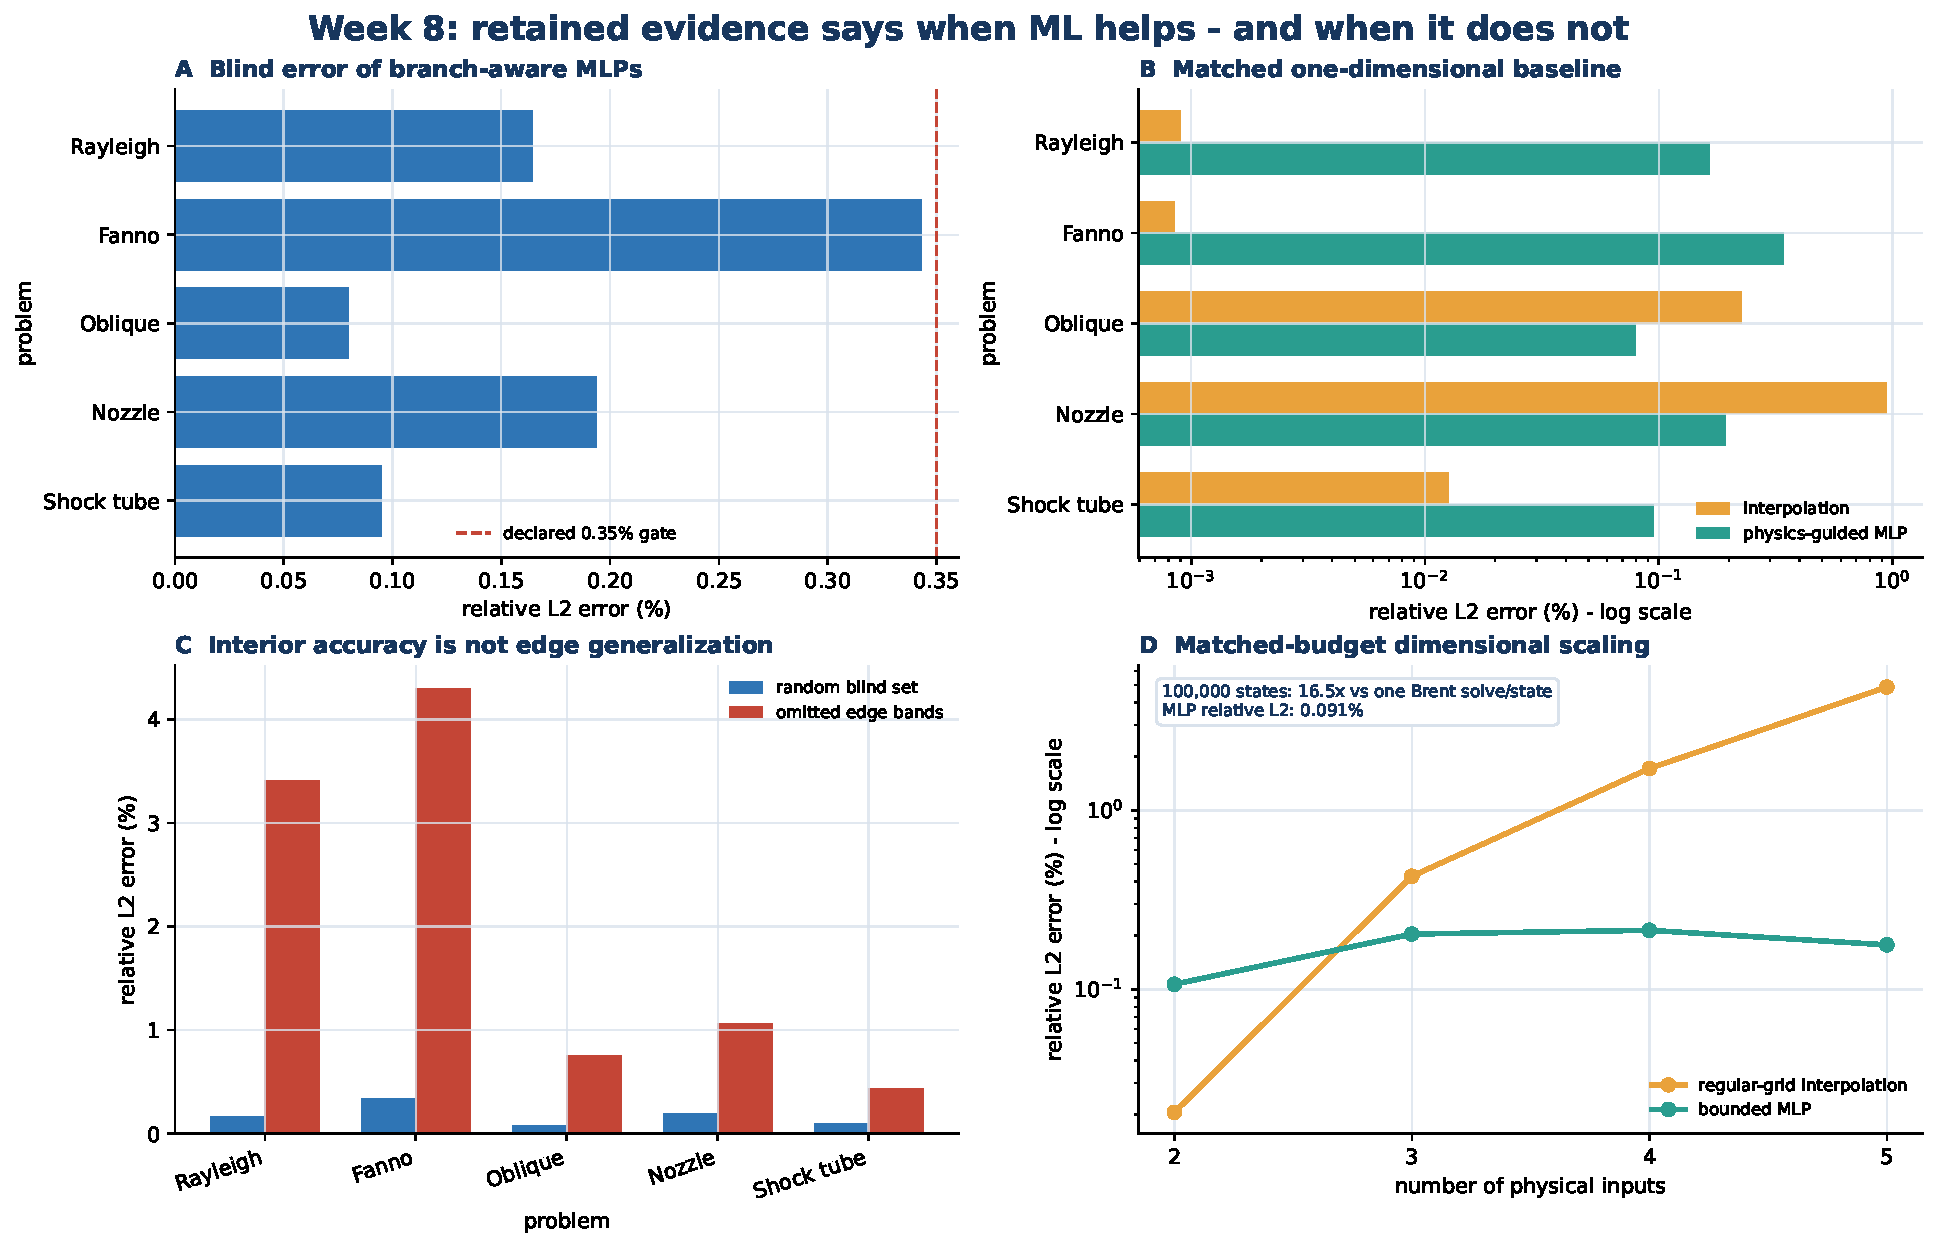
\includegraphics[width=\textwidth]{week8_model_evidence.pdf}
\caption{Retained evidence. Panel B shows why ``ML wins'' is not a general
conclusion on one-dimensional tables. Panel C separates ordinary blind accuracy
from omitted-edge testing. Panel D shows the matched-budget dimensional crossover.}
\label{fig:evidence}
\end{figure}

\subsection{The matched interpolation baseline}
For Rayleigh, Fanno, and the shock-tube table, interpolation is substantially
more accurate wherever it returns a value. It is also faster for covered
one-dimensional tables. Oblique and nozzle inverses favor the physics-guided MLP
in the retained comparison, and the MLP has complete coverage for all five tasks.

\begin{decisionbox}
Use the exact formula when it is cheap. Use interpolation for a covered
low-dimensional table when accuracy, coverage, storage, and derivatives satisfy
the application. Consider a bounded neural surrogate when repeated implicit
solves, dimensionality, compact storage, or differentiable evaluation create a
measured advantage.
\end{decisionbox}

\subsection{Edge generalization is a separate experiment}
Training on interior parameter boxes and testing only omitted low/high bands
raises relative-$L_2$ error to 3.41\% for Rayleigh, 4.30\% for Fanno, 0.755\%
for oblique shocks, 1.06\% for the nozzle, and 0.432\% for the shock tube. These
are in-domain edge tests. Calling them unrestricted extrapolation would still be incorrect.

\subsection{Dimensional scaling under matched data budgets}
With about 4096 states, a regular grid has 64 points per axis in two dimensions
but only 5 per axis in five dimensions. At five inputs, interpolation has
4.88496\% relative-$L_2$ error, while the bounded MLP has 0.177106\%. Online
interpolation remains slightly faster; the demonstrated advantage is compact
accuracy under sparse high-dimensional sampling.

That regular-grid comparison alone is not a sufficient baseline because the
MLP receives 4096 Latin-hypercube states while the grid receives only five
locations per coordinate. FlowMLLab therefore adds a local thin-plate RBF using
the same 4096 scattered training states and the same 2048 blind states. Its
errors for two through five inputs are 0.0130\%, 0.1120\%, 0.4260\%, and
0.9487\%. Thus the fairer scattered baseline closes most of the apparent gap;
the five-input MLP remains more accurate, but by a factor of about 5.4 rather
than the factor of 27.6 suggested by the regular grid alone. This added audit
is FlowMLLab teaching evidence, not a value transcribed from the manuscript.

\subsection{Application-scale timing and derivatives}
For 100,000 generalized shock-tube states in one single-thread process, the MLP
is 16.53 times faster than one Brent solve per state with 0.09148\% relative-$L_2$
error. In a nine-case nozzle inverse-design audit, safeguarded Newton iteration
converges in at most six steps, and the analytical network Jacobian agrees with
centered finite differences to $1.37\times10^{-9}$ relative difference.

\begin{warningbox}
Timing evidence is valid only for the recorded workload, implementation,
hardware environment, thread limits, warm-up, and statistic. It does not imply
that an MLP is faster than a closed-form formula or a prepared interpolation table.
\end{warningbox}

\section{Physical Diagnostics Beyond Error Norms}
Global errors must be accompanied by problem-specific checks:
\begin{center}
\begin{tabular}{p{0.22\textwidth}p{0.31\textwidth}p{0.34\textwidth}}
\toprule
Problem & Required diagnostic & Failure meaning \\
\midrule
Rayleigh & entropy trend and sonic peak location & wrong thermodynamic direction or shifted choke state \\
Fanno & nonnegative $4fL^*/D$ and sonic limit & invalid friction length or broken limiting behavior \\
Oblique shock & weak/strong branch validity and endpoints & averaged or detached state represented as attached \\
Nozzle & $1<A_s/A_t<A_e/A_t$ and back-pressure closure & shock outside nozzle or inverse mismatch \\
Shock tube & $p_2/p_1>1$ and compatibility residual & star state violates wave matching \\
\bottomrule
\end{tabular}
\end{center}
The retained evidence stores these diagnostics in CSV rather than inferring them
from visually smooth plots.

Hard bounds certify only the encoded property. For example, a valid nozzle
location does not prove back-pressure closure, and a positive shock-tube pressure
does not prove contact compatibility. The manuscript therefore reports both
validity rates and residual discrepancies; students must keep those columns separate.

\section{Bridge to Multidimensional CFD}
The Mach-3 diamond-airfoil repository contains Euler, laminar Navier--Stokes,
and SST RANS configurations at $\alpha=0^\circ,4^\circ,8^\circ$. Its two-stage
workflow uses robust first-order initialization followed by second-order MUSCL
mean-flow reconstruction. The wrapper checks more than the SU2 exit code:
\begin{enumerate}
\item fresh output and complete provenance;
\item residual history and declared reduction;
\item at least 200 force samples in the final window;
\item force-window stability and expected ranges;
\item nonphysical-point and reconstructed-state warnings;
\item symmetry and shock-angle metrics from native-grid connectivity; and
\item wall-resolution metrics where applicable.
\end{enumerate}

At the frozen Week-8 commit, the sharp-wall \texttt{euler\_alpha0} case is a
\emph{qualified teaching reference}: its forces, symmetry, shock angle, and
physicality checks are enforced, while a plateaued density residual remains an
explicit warning. The other eight cases have unresolved acceptance entries and
remain unverified.

\begin{evidencebox}
No unverified SU2 field enters the Week-8 training data. A future student project
may qualify one additional case only by predeclaring its acceptance ranges,
running a mesh/time or iteration study as appropriate, and preserving failed variants.
\end{evidencebox}

\section{Two-Lab Teaching Plan}
\subsection{Lab 1: exact gas dynamics before ML}
Students execute five references, recover both roots where applicable, close the
inverse by forward substitution, and classify all nine chapter notebooks by
numerical method. The exit ticket is a reference-solver evidence card.

\subsection{Lab 2: when should a surrogate be neural?}
Students first expose the hidden-branch failure with a small deterministic MLP.
They then inspect the five retained blind results, interpolation coverage,
omitted-edge errors, dimensional scaling, the 100,000-state workload, and
physical diagnostics. The exit ticket requires an exact/interpolation/MLP decision.

\begin{center}
\begin{tabular}{p{0.27\textwidth}p{0.55\textwidth}}
\toprule
Assessment item & Required evidence \\
\midrule
Problem definition & nondimensional input/output, domain, branch, and bound \\
Reference & equation or solver, tolerance, forward-substitution residual \\
Baseline & matched interpolation or root solve with equal information \\
Learning protocol & complete states, development-only selection, frozen gate \\
Physics & admissibility, entropy/closure/limit diagnostic \\
Generalization & blind split and a separately named edge test \\
Decision & limited claim plus one condition under which the model is rejected \\
\bottomrule
\end{tabular}
\end{center}

\section{Reproducibility Contract}
The FlowMLLab copy records source commits, continuous-integration runs, and
SHA-256 hashes for each retained CSV/JSON file. The compact Week-8 check is
\begin{verbatim}
python qa/build_week8_gas_dynamics_figures.py
python -m unittest tests.test_gas_dynamics
python qa/validate_course_release.py
\end{verbatim}
The full research regeneration remains in \texttt{GasDynamicsSciML}:
\begin{verbatim}
git checkout 374431a1033138f56e2752bf8bbf9b75a454d80c
python -m pip install -e .
python -m unittest discover -s tests -v
gasdynbench --output results/revision
\end{verbatim}
Record Python version, thread limits, seeds, workload, and evidence hashes before
comparing a regenerated result with the retained tables.

\section{Conclusions}
\begin{enumerate}
\item Exact physics defines the dataset, branch structure, bounds, and residuals.
\item A branch-hidden inverse is mathematically ill-posed; more training cannot repair it.
\item Interpolation is a required baseline and often wins on covered 1-D tables.
\item Neural value must be demonstrated through coverage, dimensional scaling,
repeated implicit workloads, compactness, or derivatives -- not assumed.
\item Edge tests, physical diagnostics, and timing protocols are separate from ordinary blind error.
\item Multidimensional CFD requires its own verification and validation chain before becoming an ML label.
\end{enumerate}

\section*{Repository and Reading Guide}
\begin{itemize}
\item E. Roohi, \emph{Introduction to Compressible Flows},
\href{https://github.com/Ehsan-Roohi/Introduction-to-Compressible-Flows}{computational companion repository}.
\item E. Roohi, \emph{GasDynamicsSciML / GasDynBench},
\href{https://github.com/Ehsan-Roohi/GasDynamicsSciML}{scientific-ML repository}.
\item E. Roohi, \emph{Physics-Guided Neural Surrogates for Canonical Compressible
Thermal-Fluid Relations}, revised manuscript \texttt{AITF-D-26-00044R1}, 2026.
\item E. Roohi, \emph{SU2 Diamond-Airfoil Verification},
\href{https://github.com/Ehsan-Roohi/SU2-Diamond-Airfoil-Verification}{teaching-CFD repository}.
\item J. D. Anderson, \emph{Modern Compressible Flow}, McGraw-Hill.
\item A. H. Shapiro, \emph{The Dynamics and Thermodynamics of Compressible Fluid Flow}, Ronald Press.
\item P. A. Thompson, \emph{Compressible-Fluid Dynamics}, McGraw-Hill.
\end{itemize}

\end{document}
